\documentclass[12pt]{article}

\usepackage{fullpage}
\usepackage{times}
\usepackage[normalem]{ulem}
\usepackage{multirow}
\usepackage{fancyhdr,graphicx,amsmath,amssymb, mathtools, scrextend, titlesec, enumitem}\usepackage[pdftex]{hyperref}
\usepackage[ruled,vlined]{algorithm2e}
\usepackage{parskip}
\usepackage{listings}
\usepackage{amsmath}
\usepackage{physics}
\usepackage{bbm}
\usepackage{titling}
\usepackage{bm}
\usepackage{geometry}
\geometry{top=1cm, left=1cm, bottom=1.5cm, right=1.5cm, margin=1cm}
\newcommand{\varvec}[2][n]{#2_1,\ldots, #2_#1}
\newcommand{\Var}{\mathrm{Var}}
\newcommand{\Bias}{\mathrm{Bias}}
\newcommand{\Cov}{\mathrm{Cov}}
\newcommand{\E}{{\rm I\kern-.3em E}}
\newcommand{\Binomial}{\mathrm{Binomial}}
\newcommand{\Bernoulli}{\mathrm{Bernoulli}}
\newcommand{\Poisson}{\mathrm{Poisson}}
\newcommand{\Normal}{\mathcal{N}}
\newcommand{\one}{\mathbbm{1}}
\newcommand{\Beta}{\text{Beta}}
\newcommand{\BetaPDF}{\text{Beta}}
\newcommand{\GammaPDF}{\text{Gamma}}
\newcommand{\Uniform}{\mathrm{Uniform}}
\newcommand{\QED}{\newline \mbox{} \hfill $\blacksquare$}
\newcommand{\Real}{\mathbb{R}}
\newcommand{\Sgn}{\mbox{Sgn}}
\renewcommand*{\arraystretch}{1.4}
\newtheorem{theorem}{Result}
\newtheorem{definition}{Definition}
\lstset{frame=tb,
	language=Python,
	aboveskip=3mm,
	belowskip=3mm,
	showstringspaces=false,
	columns=flexible,
	basicstyle={\small\ttfamily},
	numbers=none,
	stringstyle=\color{mauve},
	breaklines=true,
	breakatwhitespace=true,
	tabsize=3
}
\graphicspath{ {./figures/} }

\title{Chapter 8: Hypothesis Testing}
\begin{document}
\maketitle

\section*{Exercise 8.1}

Let $H_0$ be the hypothesis that the coin is fair, aka $\theta_0 = 0.5$.
\subsection*{Likelihood ratio test} 
The likelihood method for independent Bernoulli trial is $L(\theta | x) = \theta^{560} (1 - \theta)^{1000 - 560}$ where $560$ is the number of head. We know that $\theta=\frac{560}{1000}$ is the empirical estimator of $\theta$ that maximizes the likelihood function. So the ratio test gives 
 $$\log{\lambda(x)} = \log{\frac{  L(0.5 |x)}{L(0.56 | x)}} = 1000 \log{0.5} - \{560\log {0.56} + 440 \log {0.44}\} \Rightarrow \lambda(x) \approx  0.00073 $$

$0.00073$ is too small so $H_0$ can be rejected. Therefore the coin is not fair.

\subsection*{Check the probability of such event}
Assume coin is fair $\theta = 0.5$, then the CDF of the process is$$P(X \geq x) = \sum_{i = x}^{1000} P(X = i) = \sum_{i=x}^{1000} {1000 \choose i} 0.5^i 0.5^{1000 - i}$$

Then we can check if the event ${X \geq 560}$ is a small event for this $\theta$. Indeed it is $\approx0.08\%$. So the coin is not fair.

\section*{Exercise 8.2}
Let $H_0$ be the null hypothesis that the incident number of this year is generated from $Pois(\lambda)$ where $\lambda < 15$. To estimate whether the generating distribution has decreased in $\lambda$, we let $\pi(\lambda) = \mathcal{N}(\mu = \frac{10+15}{2} = 12.5, \sigma^2 = (15-10)^2) = \frac{1}{5 \sqrt{2 \pi}}\exp(- 0.5 \frac{(12.5 - \lambda)^2}{5^2})$ (we choose midpoint between 15 and 10 is because 10 is the MLE for the latest year's data point)

\begin{equation*}
\begin{split}
 P(\lambda < 15 | x = 10) &= \sum_{\lambda = 0}^{14} P(\lambda | x = 10) \\
  &= \frac{\sum_0^{14}  P(x= 10| \lambda)\pi(\lambda)}{\sum_0^\infty P(x=10|\lambda) \pi(\lambda)} \\
  &=  \frac{\sum_0^{14}  P(x= 10| \lambda)} {\sum_0^{30} P(x=10|\lambda)}  \left( \text{Let the prior } P(\lambda) = Uniform(0, 30) \right) \\
  &= \frac{\sum^{14}_{i = 0} i^{10} e^{-i}}{\sum^{30}_{i=0} i^{10} e^{-i}} \approx 0.87
\end{split}
\end{equation*}

Type I Error is about 1- 0.87 = 0.13, not small. If we compute $P(x <= 10 | \lambda = 15) \approx 0.11$, so $\lambda = 15$ is still capable of producing such result. It is inconclusive. 

\section*{Exercise 8.3}
$H_0$ region is $\theta \leq \theta_0$ and $H_1$'s region is $\theta > \theta_0$. Then define $b = m \theta_0$ to be the expected success count if $\theta = \theta_0$. 

A Bernoulli trial $f(y|\theta) = I_{Y=1}\theta + I_{Y=0}(1-\theta)$. Then the likelihood function $$L(\theta|y) = \prod_1^m f(y_i | \theta) ={m \choose k} \theta^k (1- \theta)^{m-k} $$ 
where $k = \sum_i Y_i$

To maximize $L$, we can use the MLE which is the $\theta_{\text{max}} = \frac{k}{m}$. To reject $H_0$, we need the MLE to stay out $H_0$ region, so $\frac{k}{m} > \theta_0 \Rightarrow  \sum_i Y_i = k > m\theta_0 = b$ 


\section*{Exercise 8.5}

\textbf{(a)} The likelihood function $$L(\theta, v|x) = \prod_{i=1}^n f(x_i |\theta, v) = \frac{\theta^n  v^{n\theta}}{(\prod_i x_i)^{\theta+1}} \prod_i I_{\left[v, \infty\right)}(x_i) = \frac{\theta^n  v^{n\theta}}{(\prod_i x_i)^{\theta+1}}, (\text{given } v \leq x_{\text{min}}, 0 {\text{ otherwise}})$$

Holding $\theta$ fixed, $L$ is a monotonic polynomial function of $v$. So $v_0 = x_{(1)}$ the boundary of $v$ maximizes $L$. 

Let $\frac{\partial \log L}{\partial \theta} = \frac{n}{\theta} + \log(x_{(1)}^n) - \log(\prod_i x_i) = 0$, then we get $$\theta_0 = \frac{n}{\log \left( \frac{ \prod_i x_i}{x_{(1)}^n}\right)} = \frac{n}{T(x)}$$

where $T \equiv  \log \left( \frac{ \prod_i x_i}{x_{(1)}^n}\right)$

\textbf{(b)} $H_0 = \{(\theta = 1, v)\}$,
So the rejection region of $H_0$ is $$\lambda(x) = \frac{\sup_{\theta=1} L(\theta, v| x)}{\sup_{\theta} L(\theta, v | x)} = \frac{T^n}{n^n}\exp(n - T) \leq c$$ 

We take derivative of $\lambda$,  $$\partial_{T}\lambda = \left(\frac{T}{n}\right)^{n-1} e^{n-T} \left( 1- \frac{T}{n} \right)$$ 

So the monotonicity of $\lambda$ is determined by $(1 - T/n)$. When $T = n$, $\lambda$ reaches maximum of 1, when $T < n$, $\lambda$ increases monotonically and when $T > n$, $\lambda$ decreases monotonically. Therefore, if $\lambda(x) < c$ for $0 < c \leq 1$, we will have two values $c_1$ and $c_2$ (on left/right side of $n$ respectively) where $T \leq c_1 \leq n$ or $n \leq c_2 \leq T$.

\section*{Exercise 8.6}
(a) Let $$L(\theta, \mu|x, y) = f(x_1, \ldots, x_n, y_1, \ldots, y_m | \theta, \mu) = \prod_i^n f(x_i|\theta) \prod_i^m f(y_i|\mu) = \theta^n \mu^m \exp(-\theta \sum_i^n x_i - \mu \sum_i^m y_i)$$ be the likelihood function of the joint distribution. Then 
$$ \ln(L(\theta, \mu)) = n\ln(\theta) + m \ln(\mu) -\theta \sum_i^n x_i - \mu \sum_i^m y_i$$.
For $H_0$ where $\theta = \mu$, we solve $\frac{d\ln(L(\theta, \mu | \theta = \mu))}{d\theta} =0$ and get $$\hat{\theta_0} = \frac{n+m}{\sum_i^n x_i + \sum_i^m y_i}$$ as the MLE under the constraint.

For $H_1$,  we solve $\frac{\partial \ln L}{\partial \theta} = 0$ and $\frac{\partial \ln L }{\partial \mu} = 0$ and get $$\hat{\theta_1} = \frac{n}{\sum_i^n x_i},  \quad \hat{\mu_1} = \frac{n}{\sum_i^m y_i}$$.

Therefore $$\lambda((x, y)) = \frac{\sup_{\theta=\mu} L(\theta, \mu|x, y)}{\sup_{\theta, \mu} L(\theta, \mu|x, y)} = \frac{ L(\hat{\theta_0}, \hat{\theta_0}|x, y)}{L(\hat{\theta_1}, \hat{\mu_1})} = \frac{(n+m)^{n+m}}{n^nm^m}\frac{\left(\sum_i^nx_i\right)^n \left(\sum_i^m y_i\right)^m}{\left(\sum_i^nx_i +  \sum_i^m y_i \right)^{n+m}}$$

(b) To show that $T = \frac{\sum X}{\sum X + \sum Y}$ can also give the same LRT, we just need to express the LRT in terms of $T$. Let $C= \frac{(n+m)^{n+m}}{n^nm^m}$, then
$$\lambda((x, y)) =C \frac{\left(\sum_i^nx_i\right)^n \left(\sum_i^m y_i\right)^m}{\left(\sum_i^nx_i +  \sum_i^m y_i \right)^{n+m}} 
= C  \left(\frac{\sum_i^nx_i}{\sum_i^nx_i +  \sum_i^m y_i}\right)^n \left(\frac{\sum_i^m y_i}{\sum_i^nx_i +  \sum_i^m y_i}\right)^m  = C T^n (1 - T)^m $$

(c)
Let $U = \sum^{n}_{1} X_i$, then we calculate the MGF,  $M_U(t) = E\left[e^{\sum_i t}\right] = \prod E\left[e^{X_it}\right]=\prod M_{X_i}(t) = \frac{1}{(1 - \theta t)^n}$ since $H_0$ is true. It matches the gammar distribution's MGF, therefore $U = \sum_i X_i \sim \GammaPDF(n, \theta)$. Similarly $V = \sum^m_1 Y_i \sim \GammaPDF(m, \theta)$.

Next is to find the distribution of $T  = \frac{U}{U + V}$. Since $U, V$ are independent, so $$f(u, v) = f(u) f(v) = \GammaPDF(n, \theta)\GammaPDF(m, \theta) = \frac{1}{\Gamma(n)\Gamma(m) \theta^{n+m}} u^{n-1}v^{m-1} e^{-\frac{1}{\theta}(u + v)}$$

Let $S = U + V$, then $T = \frac{U}{U + V} = \frac{U}{S}$. We have $U = TS,  V = S(1-T)$. So the Jacobian $|J| = |S|$. By change of variables, we have 
$$ g(t, s) = f(u(t, s)) f(v(t, s)) |J| = \frac{1}{\Gamma(n)\Gamma(m) \theta^{n+m}} t^{n-1}(1-t)^{m-1} s^{n + m-1} e^{-\frac{1}{\theta}s}$$
Next we maginalize $s$, 
\begin{equation*}
 \begin{split}
	g(t) &= \int_{0}^{\infty} g(t, s) ds =  \frac{1}{\Gamma(n)\Gamma(m)\theta^{n+m}}  t^{n-1}(1-t)^{m-1} \int_{0}^{\infty} s^{n + m-1} e^{-\frac{1}{\theta}s}ds \\ 
	&= \frac{\Gamma(n+m)}{\Gamma(n)\Gamma(m)} t^{n-1}(1-t)^{m-1} \int_0^\infty \frac{1}{\Gamma(n + m) \theta^{n+m}} s^{n + m-1} e^{-\frac{1}{\theta}s}ds \\
	&=  \frac{\Gamma(n+m)}{\Gamma(n)\Gamma(m)} t^{n-1}(1-t)^{m-1} \\
	&= \BetaPDF(n, m)
\end{split}
\end{equation*}

\section*{Exercise 8.7}
(a)
 For the integration of the pdf to converge, $\lambda > 0$.
 \begin{align*}
	LRT(x) = \frac{\sup_{\theta \leq 0, \lambda} L(\lambda, \theta | x)}{\sup_{\theta, \lambda} L(\lambda, \theta | x)} = \frac{\sup_{\theta \leq 0, \lambda}\frac{1}{\lambda^n} \exp(- \frac{1}{\lambda} \sum_i (x_i - \theta)) I(\theta \leq x_{(1)})}{\sup_{\theta, \lambda}\frac{1}{\lambda^n}  \exp(- \frac{1}{\lambda} \sum_i (x_i - \theta)) I(\theta \leq x_{(1)}) } 
\end{align*}
Let $f(\theta, \lambda) = \frac{1}{\lambda^n} \exp(- \frac{1}{\lambda} \sum_i (x_i - \theta)) $ and $\log f = -n\log \lambda - \frac{1}{\lambda} \sum_i (x_i - \theta)$. Take the partial derivative wrt $\theta$, $\frac{\partial \log f}{\partial \theta} = \frac{n\theta}{\lambda}$ which means $f$ is a monotonic increasing function along $\theta$ (attains maximum at $\theta = 0$). 

Let $g(\theta, \lambda) = f(\theta, \lambda) I(\theta \leq x_{(1)})$, then $g(\theta, \lambda)$ attains maximum at $\theta = x_{(1)}$ holding $\lambda$ fixed.  Then we have $g(x_{(1)}, \lambda) = \frac{1}{\lambda^n} \exp(- \frac{1}{\lambda} \sum_i (x_i - x_{(1)})))$

Next we take the deritvative wrt to $\lambda$,  $\frac{\partial \log g(x_{(1)}, \lambda)}{\partial \lambda} = -\frac{n}{\lambda} + \frac{\sum_i (x_i -  x_{(1)})}{\lambda^2} = 0$ implies when $\lambda = \bar{x} - x_{(1)}$, $g(x_{(1)}, \lambda)$ attains maximum. 

Now we have
$$\sup_{\theta, \lambda}\frac{1}{\lambda^n}  \exp(- \frac{1}{\lambda} \sum_i (x_i - \theta)) I(\theta \leq x_{(1)}) = g(x_{(1)}, \bar{x} - x_{(1)})$$

If we constrain $\theta \leq 0$,  then by the same computation, $g$ will attain maximum when $\theta = \min(0, x_{(1)})$ and $\lambda = \bar{x} - \min(0, x_{(1)})$.

Now we can write the LRT as 
\begin{align*}
	LRT(x) &=  \frac{\sup_{\theta \leq 0, \lambda} L(\lambda, \theta | x)}{\sup_{\theta, \lambda} L(\lambda, \theta | x)} \\
	&=  \frac{g(\min(0, x_{(1)}), \bar{x} - \min(0, x_{(1)}))}{g(x_{(1)}, \bar{x} - x_{(1)})} \\
	&= \begin{cases*}
		1 &  $x_{(1)} < 0$ \\
		\left(1 - \frac{x_{(1)}}{\bar{x}} \right)^n & $x_{(1)} \geq 0 $
	\end{cases*}
\end{align*}

\section*{Exercise 8.12}
(a) By Exercise 8.37 below, when $\sigma^2$ is known, we can write the power function of the test as 
$$ \beta(\mu) = P_\mu(X \in R) = P_\mu(\overline{X} > 0 + z_\alpha \frac{\sigma}{\sqrt{n}}) $$
where $P(Z > z_alpha) = z_\alpha$. By subtracting both side with $\mu$, we have 
$$ \beta(\mu) =  P_\mu( \frac{\overline{X} - \mu}{ \frac{\sigma}{\sqrt{n}}} > z_\alpha - \frac{\mu}{ \frac{\sigma}{\sqrt{n}}}) = P_\mu(Z > z_\alpha - \frac{\mu}{ \sigma / \sqrt{n}})$$
Now we can plot the value of the power function for each $\mu \in [-1, 2]$.

\begin{lstlisting}[language=Python]
	import numpy as np
	import scipy.stats as st
	import matplotlib.pyplot as plt
	
	sigma = 1
	samples = [1, 4, 16, 64, 100]
	test_size = 0.05
	z_test_size = st.norm.ppf(1 - test_size)
	
	def get_power_fun(n):
	return lambda mean: 1 - st.norm.cdf(z_test_size - mean / (sigma / np.sqrt(n)))
	
	data = []
	mean_range = np.linspace(-1.2, 2, num=100)
	
	ax = plt.subplot()
	for n in samples:
	values = get_power_fun(n)(mean_range)
	ax.plot(mean_range, values, label=f"sample size={n}")
	
	ax.set_title="Power function by sample sizes"
	ax.set_ylabel("power function")
	ax.set_xlabel("sample mean")
	ax.legend()
\end{lstlisting}
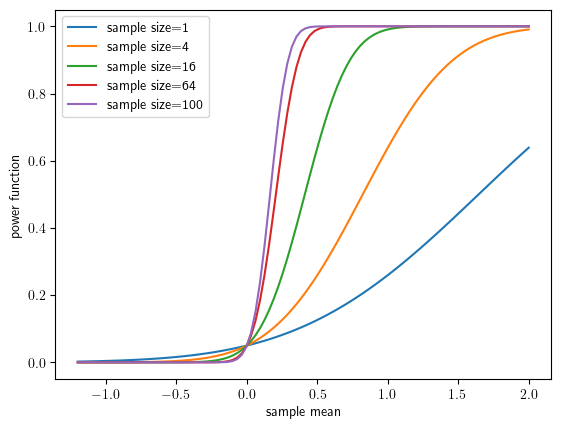
\includegraphics{fig_ch_08_12_a}

\section*{Exercise 8.37}
(a) 
Given $Z \sim \Normal(0, 1)$ and $P(Z > z_\alpha) = \alpha$,  Consider \begin{align*}
	&\sup_{\theta \in \Theta_0} P_{\theta}\left( \overline{X} > \theta_0 + z_{\alpha}\frac{\sigma}{ \sqrt{n}} \right) \\
	&\sup_{\theta \in \Theta_0} P_{\theta}\left( \frac{\overline{X} - \theta}{\sigma / \sqrt{n}} > \frac{\theta_0 - \theta}{\sigma / \sqrt{n}} + z_{\alpha} \right) \\
	&\sup_{\theta \leq \theta_0} P_{\theta}\left( z > \frac{\theta_0 - \theta}{\sigma / \sqrt{n}} + z_{\alpha} \right) \\
\end{align*}
the above probability is an increasing function of $\theta$ when $\theta \leq \theta_0$, therefore
$$
 \sup_{\theta \leq \theta_0} P_{\theta}\left( z > \frac{\theta_0 - \theta}{\sigma / \sqrt{n}} + z_{\alpha} \right) = P_{\theta_0}(z > z_\alpha) = \alpha \\
$$
So $ \overline{X} > \theta_0 + z_{\alpha}\frac{\sigma}{ \sqrt{n}} $ is indeed a test of size $\alpha$ that rejects $H_0$.  \QED

To derive the test from LRT is, we have $$
\begin{aligned}
	\lambda(x) &= \frac{\sup_{\theta \leq \theta_0} L(x, | \theta, \sigma^2) }{\sup_{\theta \leq \theta_0} L(x, | \theta, \sigma^2)} 
   = \frac{\exp{-\frac{1}{2\sigma^2} \sum (x_i - \min(\bar{x}, \theta_0))^2 }}{\exp{-\frac{1}{2\sigma^2} \sum (x_i - \theta_0)^2 }}  \\
    &= \begin{cases*}
	      	1,                                                      & $\theta_0 = \min(\overline{x}, \theta_0)$ \\
	      	\exp{-\frac{n}{2\sigma^2}(\overline{x} - \theta_0)^2 }, & $\overline{x} = \min(\overline{x}, \theta_0)$ \\
    \end{cases*}\\
\end{aligned}
$$
The rejection region for $H_0$ is $\{x\in R | \lambda(x) < c\}$ for $c \in [0, 1]$.  We can write  \begin{align*}
		& \sup_{\theta \leq \theta_0} P (x \in R) \\
		&\Rightarrow \sup_{\theta \leq \theta_0} P (\lambda(x) < c) \\
		&\Rightarrow \sup_{\theta \leq \theta_0} P\left(\exp{-\frac{n}{2\sigma^2}(\overline{x} - \theta_0)^2 }  < c\right)  \\
		&\Rightarrow \sup_{\theta \leq \theta_0} P\left(\overline{x} > \theta_0 + \frac{\sigma}{\sqrt{n}}\sqrt{2\ln(1/c)} \right) \\ 
		&\Rightarrow \sup_{\theta \leq \theta_0} P\left(\overline{x} > \theta_0 + \frac{\sigma}{\sqrt{n}}z_\alpha \right)  \quad \quad, (\text{Simply choose } z_\alpha \equiv \sqrt{2\ln(1/c)}) \\
		&\Rightarrow \sup_{\theta \leq \theta_0} P\left( \frac{\overline{X} - \theta}{\sigma / \sqrt{n}} > \frac{\theta_0 - \theta}{\sigma / \sqrt{n}} + z_{\alpha} \right) \\
		&\Rightarrow \sup_{\theta \leq \theta_0} P\left( z > \frac{\theta_0 - \theta}{\sigma / \sqrt{n}} + z_{\alpha} \right), \quad \quad (Z \sim \Normal(0, 1)) \\
		&\Rightarrow P\left( z > z_{\alpha} \right) = \alpha
\end{align*}

\end{document}